% !TeX encoding = UTF-8
% !TeX spellcheck = pt_BR
% !TeX root = 20201-CODDISC-JOAO-FERREIRA.tex
% ------------------------------------------------------------------------------

% ------------------------------------------------------------------------------
% Template para aulas da UNINASSAU
% Autor: João Ferreira da Silva Júnior
% Versão: 0.2 - 2021-09-12
% ------------------------------------------------------------------------------



% ------------------------------------------------------------------------------
% ------------------------------------------------------------------------------
% ------------------------------------------------------------------------------
% ------------------------------------------------------------------------------
% ------------------------------------------------------------------------------
% ------------------------------------------------------------------------------
% ------------------------------------------------------------------------------
% ------------------------------------------------------------------------------
% ------------------------------------------------------------------------------
% ------------------------------------------------------------------------------
\section[Planejamento da Disciplina]{Planejamento da Disciplina}\label{sec:sec03}



{\usebackgroundtemplate{{\transparent{0.2}\includegraphics[width=\paperwidth,height=\paperheight,keepaspectratio]{img/logo/background-branco.png}}}
  % \begin{frame}[allowframebreaks,t]%\frametitle{ ---}
  \begin{frame}[plain]%\frametitle{}

    \vfill
    \centering

    \addtobeamertemplate{block begin}{\pgfsetfillopacity{0.5}}{\pgfsetfillopacity{1}}
    % \setbeamercolor{block title}{use=structure,fg=white,bg=blue}
    \setbeamercolor{block body}{use=structure,fg=black,bg=blue!50!white}
    \begin{block}{}
      \centering{}
      \Huge{\textbf{Planejamento da Disciplina}}
    \end{block}

    \vfill

  \end{frame}
} % usebackgroundtemplate



% ------------------------------------------------------------------------------
% ------------------------------------------------------------------------------
% ------------------------------------------------------------------------------
% ------------------------------------------------------------------------------
% ------------------------------------------------------------------------------
\subsection[Calendário Acadêmico]{Calendário Acadêmico}\label{subsec:sec03-calendario-academico}



% \begin{frame}[allowframebreaks,t]\frametitle{Calendário Acadêmico ---}
\begin{frame}[t]\frametitle{Calendário Acadêmico}

  \begin{figure}[htb]
    \centering{}
    % \includegraphics[trim=left bottom right top, clip]{file}
    % trim={<left> <lower> <right> <upper>},clip
    % 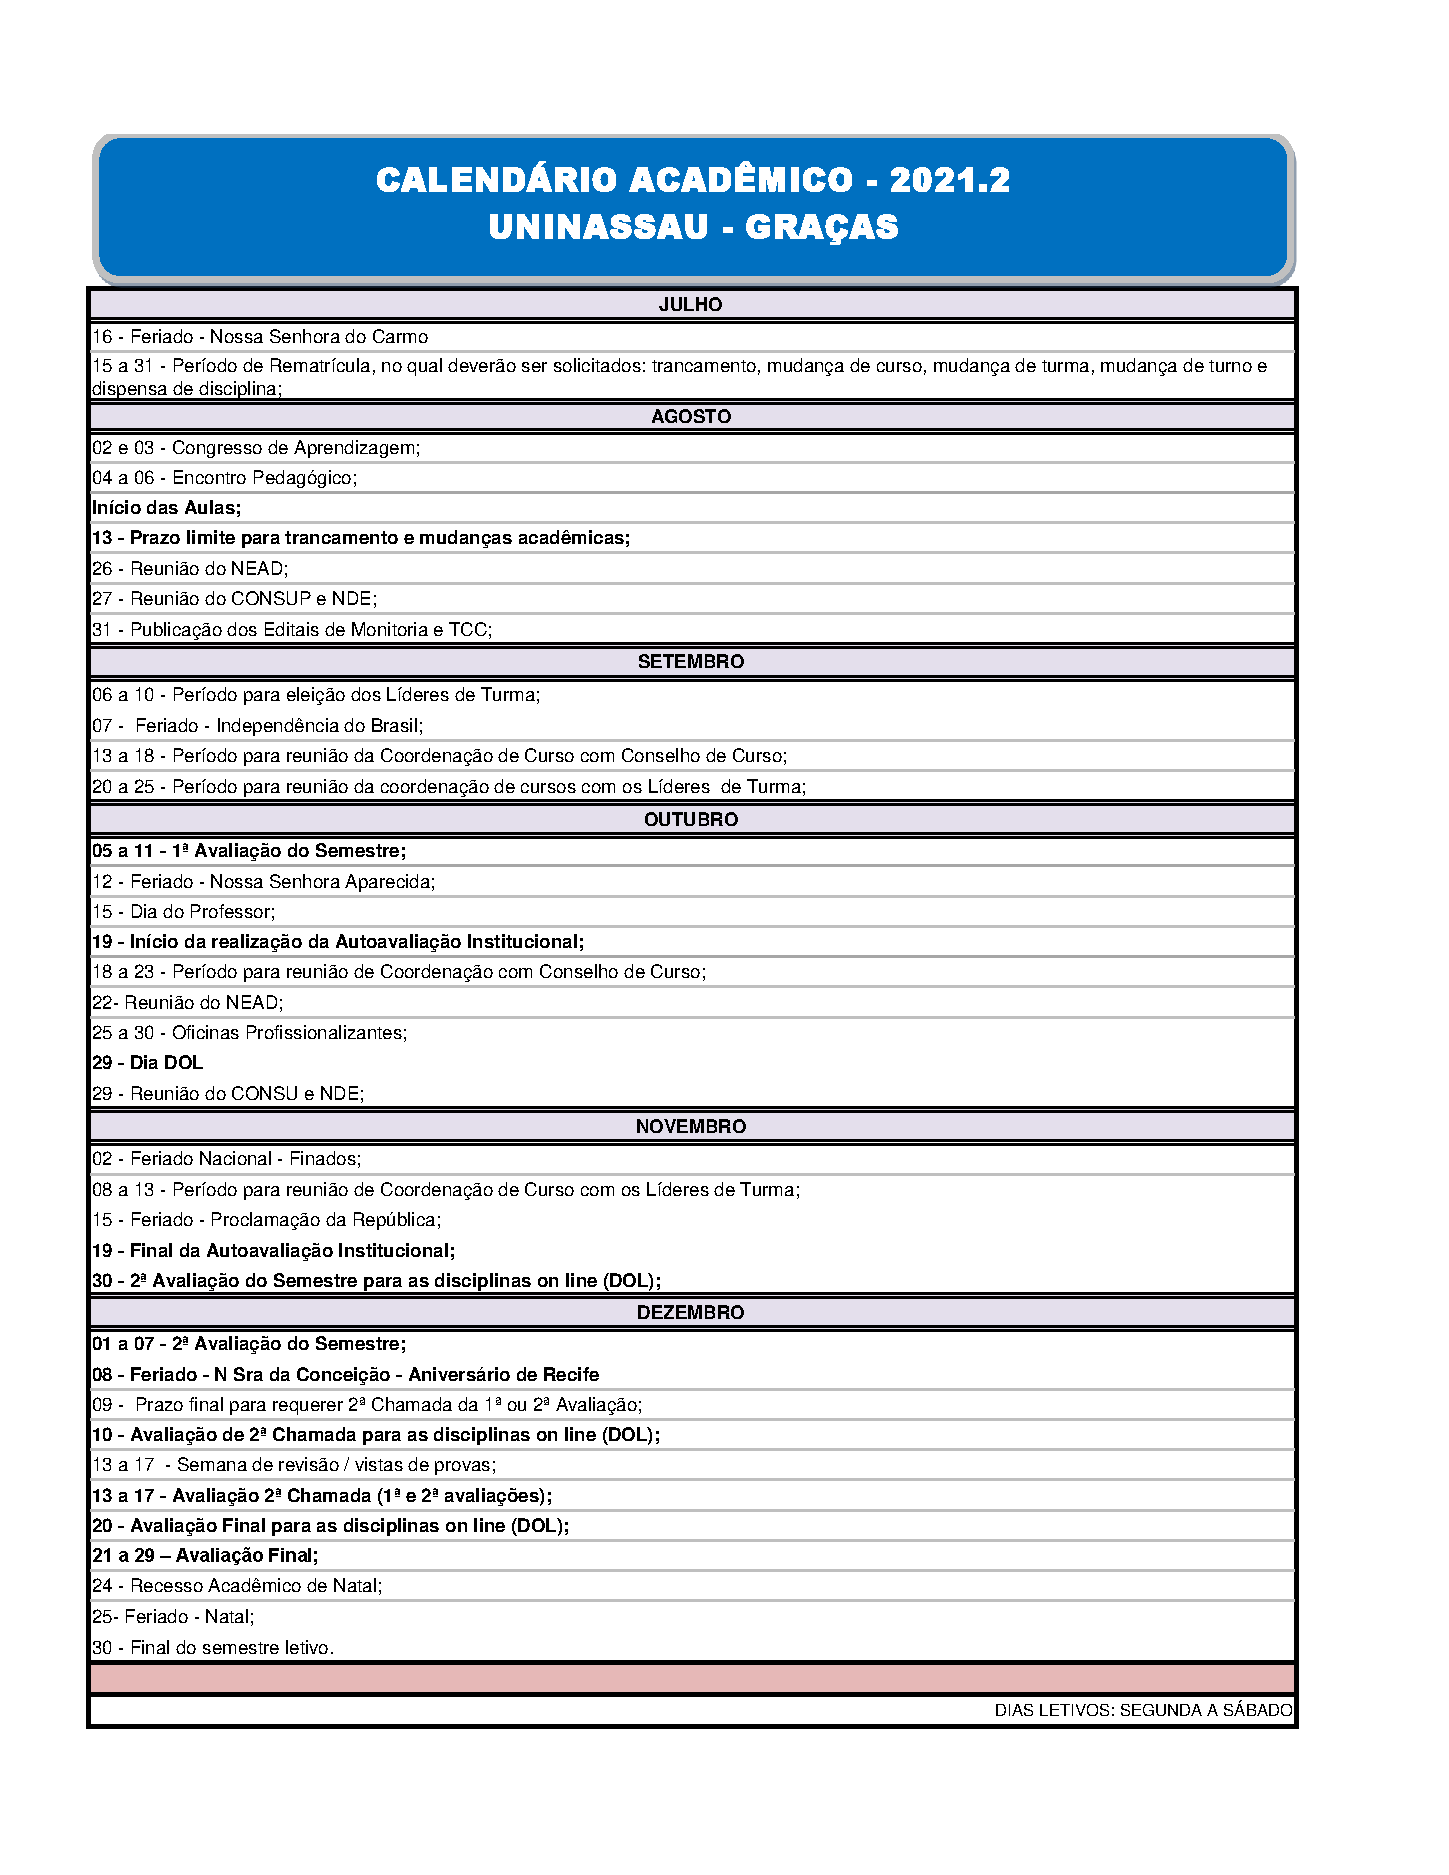
\includegraphics[width=0.9\linewidth,keepaspectratio,trim={40px 620px 70px 65px},clip]{img/sec03/calendario-academico.pdf}
    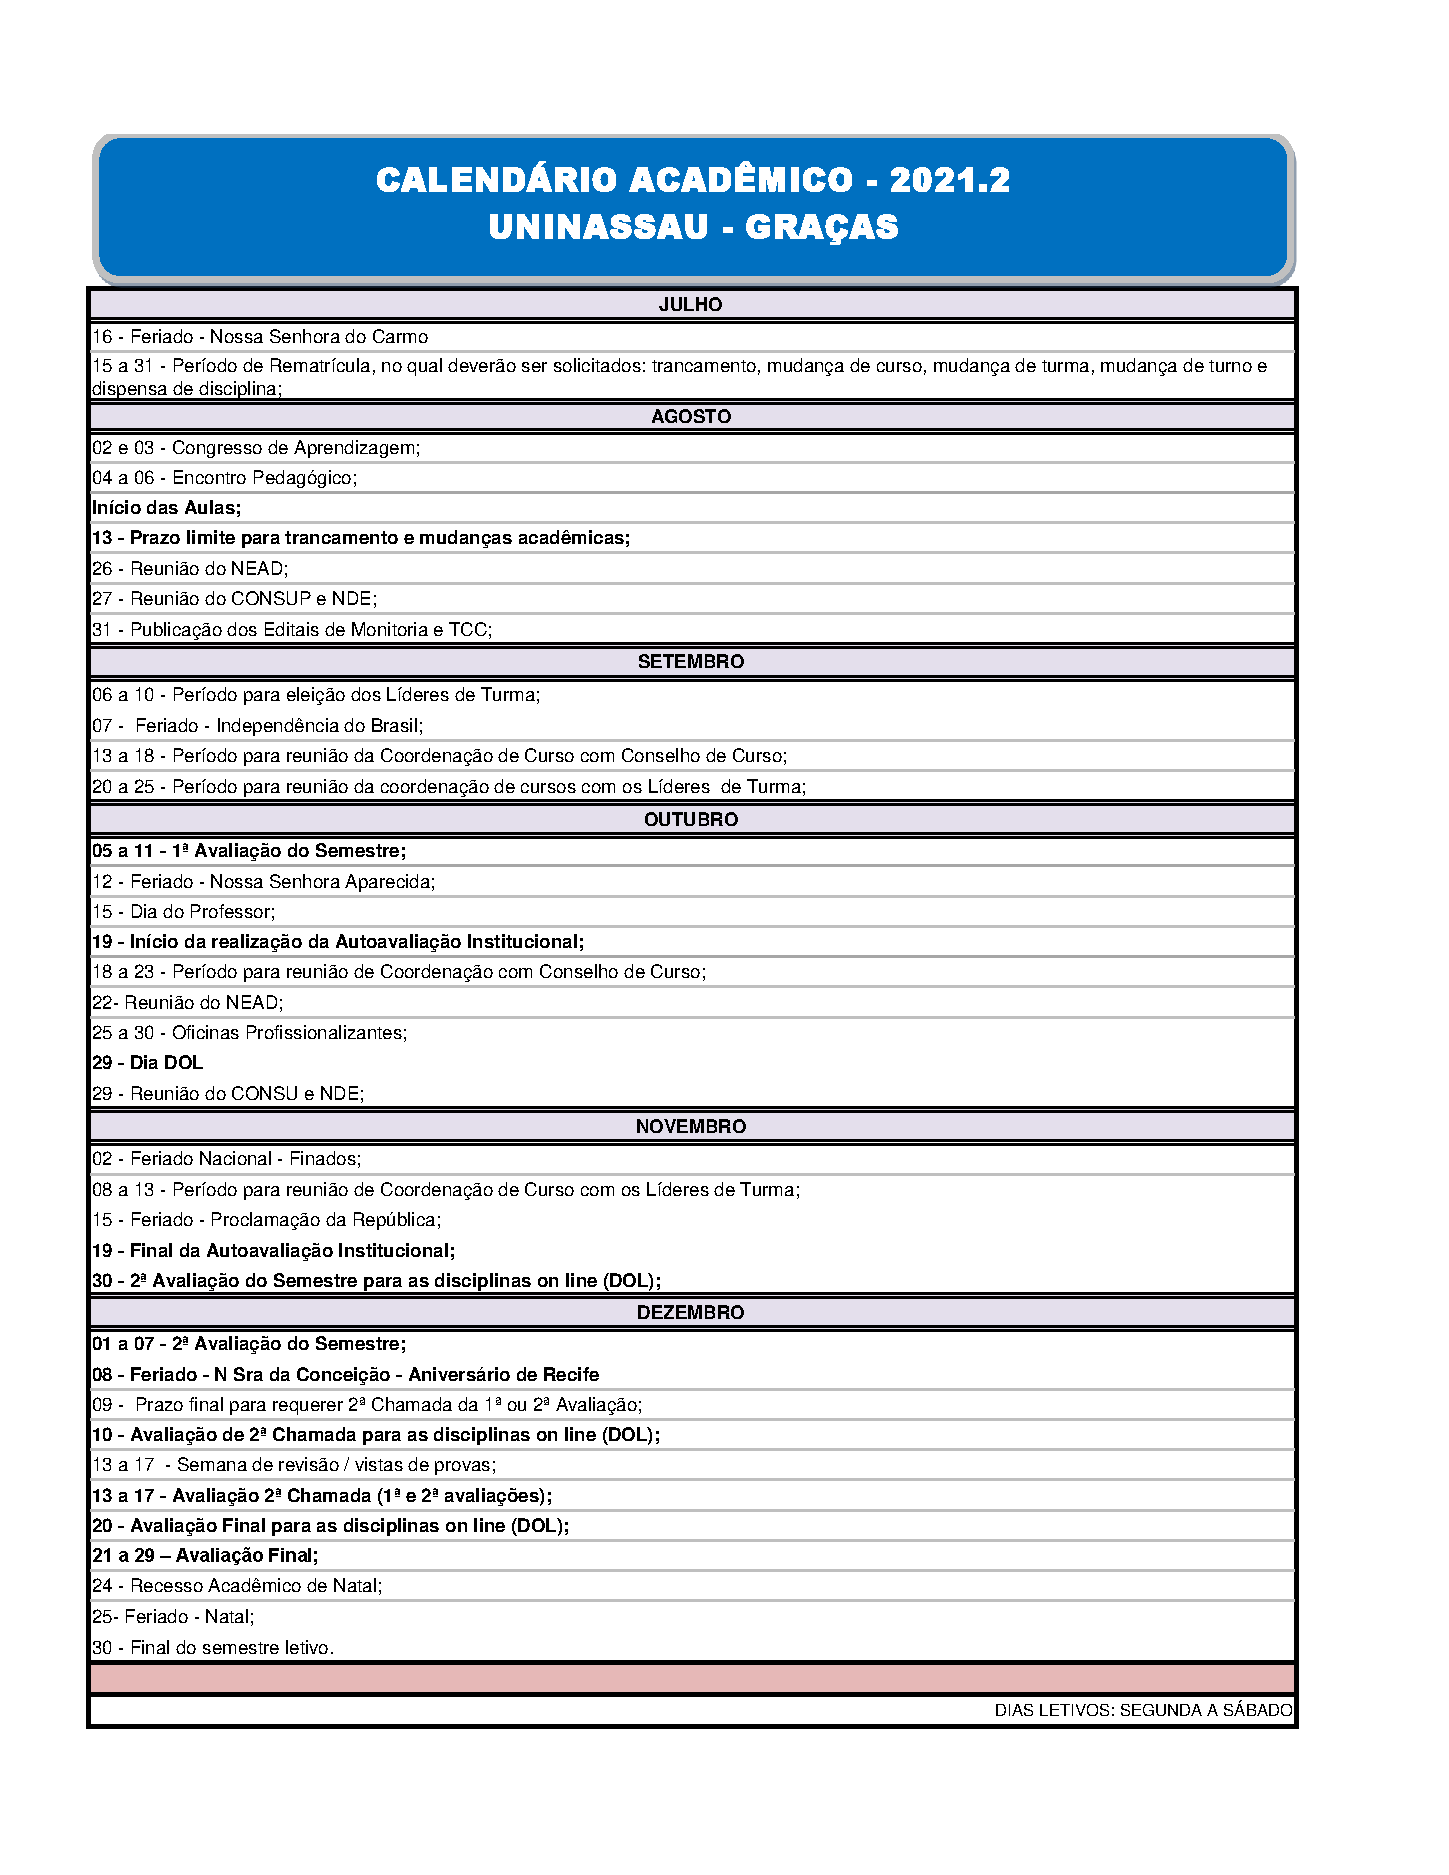
\includegraphics[height=0.85\textheight,keepaspectratio]{img/sec03/calendario-academico.pdf}
  \end{figure}

\end{frame}



% ------------------------------------------------------------------------------
% ------------------------------------------------------------------------------
% ------------------------------------------------------------------------------
% ------------------------------------------------------------------------------
% ------------------------------------------------------------------------------
\subsection[Participação]{Participação}\label{subsec:sec03-participacao}



% \begin{frame}[allowframebreaks,t]\frametitle{Participação ---}
\begin{frame}[t]\frametitle{Participação}

  \begin{itemize}
    \justifying{}
    \setlength\itemsep{1em}
    \item Frequência mínima de 75\% das aulas, faltas reprovam. Determinação institucional.
    \item Participação em aula e interação positiva entre os alunos.
    \item Questionamentos pertinentes e ajuda a demais colegas de turma.
    \item Adequação ao conteúdo ministrado e contexto da disciplina.
  \end{itemize}

\end{frame}



% ------------------------------------------------------------------------------
% ------------------------------------------------------------------------------
% ------------------------------------------------------------------------------
% ------------------------------------------------------------------------------
% ------------------------------------------------------------------------------
\subsection[Lista de Exercícios]{Lista de Exercícios}\label{subsec:sec03-lista-exercicios}



% \begin{frame}[allowframebreaks,t]\frametitle{Lista de Exercícios ---}
\begin{frame}[t]\frametitle{Lista de Exercícios}

  \begin{itemize}
    \justifying{}
    \setlength\itemsep{1em}
    \item Poderá, ou não, haver listas de exercícios, que irão valer ponto e servirão como base de estudo, mas não de todo o conteúdo ministrado, para as avaliações.
    \item A(s) lista(s) de exercícios aplicadas até a primeira avaliação, terão conteúdo relacionado que contará eventual pontuação para esta.
    \item A(s) lista(s) de exercícios aplicadas após a primeira avaliação e até a segunda avaliação, terão conteúdo relacionádo e contará eventual pontuação para esta.
    \item Nenhuma eventual pontuação valerá para a segunda chamada ou prova final.
    \item Cada lista de exercício aplicada valerá ponto a ser adicionado à nota da respectiva avaliação.
  \end{itemize}

\end{frame}



% ------------------------------------------------------------------------------
% ------------------------------------------------------------------------------
% ------------------------------------------------------------------------------
% ------------------------------------------------------------------------------
% ------------------------------------------------------------------------------
\subsection[Projeto da Disciplina]{Projeto da Disciplina}\label{subsec:sec03-projeto-disciplina}



% \begin{frame}[allowframebreaks,t]\frametitle{Projeto da Disciplina ---}
\begin{frame}[t]\frametitle{Projeto da Disciplina}

  \begin{itemize}
    \justifying{}
    \setlength\itemsep{1em}
    \item Será voltado à aplicação dos conceitos aprendidos em sala de aula, nas listas de exercícios e na bibliografia da disciplina que consta na ementa ou nesta apresentação.
    \item Poderá ser feito individualmente ou em grupo, mas atentem ao fato de que aleatoriamente serão feitoso questionamentos a qualquer um dos membros, e, na incapacidade de resposta, a falha será atribuída a todo o grupo.
    \item A(s) lista(s) de exercícios apicadas após a primeira avaliação e até a segunda avaliação, terá conteúdo relacionádo e contará eventual pontuação para esta.
    \item O projeto será avaliado em apresentação para toda a turma, quando deverão ser demonstrados todos os processos desenvolvidos na pesquisa e elaboração, bem como o eventual funcionamento do projeto.
  \end{itemize}

\end{frame}



% ------------------------------------------------------------------------------
% ------------------------------------------------------------------------------
% ------------------------------------------------------------------------------
% ------------------------------------------------------------------------------
% ------------------------------------------------------------------------------
\subsection[Avaliações]{Avaliações}\label{subsec:sec03-avaliacoes}



% \begin{frame}[allowframebreaks,t]\frametitle{Avaliações ---}
\begin{frame}[t]\frametitle{Avaliações}

  \begin{itemize}
    \justifying{}
    \setlength\itemsep{1em}
    \item 1ª avaliação:
    \begin{itemize}
      \justifying{}
      \item Data:
      \item Forma: Avaliação realizada na ferramenta Microsoft Teams.
    \end{itemize}
    \item 2ª avaliação:
    \begin{itemize}
      \justifying{}
      \item Data:
      \item Forma: Avaliação realizada na ferramenta Microsoft Teams.
    \end{itemize}
    \item 2ª chamada:
    \begin{itemize}
      \justifying{}
      \item Data:
      \item Forma: Avaliação realizada na ferramenta Microsoft Teams.
    \end{itemize}
    \item Prova final:
    \begin{itemize}
      \justifying{}
      \item Data:
      \item Forma: Avaliação realizada na ferramenta Microsoft Teams.
    \end{itemize}
  \end{itemize}

\end{frame}



% ------------------------------------------------------------------------------
% ------------------------------------------------------------------------------
% ------------------------------------------------------------------------------
% ------------------------------------------------------------------------------
% ------------------------------------------------------------------------------
\subsection[Comunicação da Turma]{Comunicação da Turma}\label{subsec:sec03-comunicacao-turma}



% \begin{frame}[allowframebreaks,t]\frametitle{Comunicação da Turma ---}
\begin{frame}[t]\frametitle{Comunicação da Turma}

  \begin{figure}[htb]
    \centering{}
    \includegraphics[width=0.07\paperwidth]{img/sec03/telegram.png}

    \textbf{\href{https://telegram.org}{Telegram}}
  \end{figure}

  \begin{columns}
    \begin{column}{0.45\linewidth}
      \textbf{Vantagens:}
      \begin{itemize}
        \justifying{}
        \setlength\itemsep{1em}
        \item Grupo pode ter muitos membros e a troca de arquivos é bem otimizada.
        \item Histórico permanente, quem entre depois poderá ver todas as mensagens já trocadas no grupo.
        \item Ótimo aplicativo para desktop/web.
      \end{itemize}
    \end{column}

    \begin{column}{0.45\linewidth}
      \textbf{Disponível para:}
      \begin{itemize}
        \justifying{}
        % \setlength\itemsep{1em}
        \item \href{https://telegram.org/dl/android}{Android}
        \item \href{https://telegram.org/dl/ios}{iPhone/iPad}
        \item \href{https://desktop.telegram.org}{PC/Mac/Linux}
        \item \href{https://web.telegram.org}{Web}
        \item \href{https://macos.telegram.org}{macOS}
      \end{itemize}

      \textbf{Link para participar o Telegram:}

      \href{https://web.telegram.org}{https://web.telegram.org}
    \end{column}
  \end{columns}

\end{frame}
